\documentclass[letterpaper]{article}
\usepackage{calc,amsmath,amssymb,amsfonts}
\usepackage[LGR,T1]{fontenc}
\usepackage[greek,english]{babel}
\usepackage{xcolor,longfbox,fancyhdr}
\usepackage[margin=1in,noheadfoot]{geometry}
\usepackage{array,supertabular,hhline,enumitem,hyperref}
\hypersetup{colorlinks=true,allcolors=blue,pdfauthor=Pham Hai Nam}
\usepackage[pdftex]{graphicx}
\makeatletter\newdimen\@tempdimd\makeatother
% Outline numbering
\setcounter{secnumdepth}{0}
\makeatletter
\newcommand\arraybslash{\let\\\@arraycr}
\makeatother
% Pages
\fancypagestyle{Standard}{\fancyhf{}
  \fancyhead[L]{}
  \fancyfoot[L]{}
  \renewcommand\headrulewidth{0pt}
  \renewcommand\footrulewidth{0pt}
  \renewcommand\thepage{\arabic{page}}
}
\pagestyle{Standard}
\setlength\tabcolsep{1mm}
\renewcommand\arraystretch{1.3}
\author{Pham Hai Nam}
\date{2024-10-18}
\begin{document}
\clearpage
\pagestyle{Standard}
{\centering
\textcolor{black}{Machine Learning 2024 Project Midterm Report}
\par}

{\centering
\textcolor{black}{Do Duc Truong, Tran Minh Duc, Pham Hai Nam}
\par}


\bigskip

\textbf{\textcolor{black}{Part A: Machine Learning Models }}

\textbf{\textcolor{black}{4.1  k-Nearest Neighbor (KNN)}}\textbf{\textcolor{black}{\ \ }}\textbf{\textcolor{black}{
}}\textbf{\textcolor{black}{\ \ }}\textbf{\textcolor{black}{
}}\textbf{\textcolor{black}{\ \ }}\textbf{\textcolor{black}{ }}\textbf{\textcolor{black}{\ \ \ \ }}

\begin{itemize}[series=listWWNumi,label=[F0B7?]]
\item \textbf{\textcolor{black}{Step 2:}}\textcolor{black}{ To observe how the accuracy of predictions changes with
different numbers of nearest neighbors we vary the value of k to (k = 1, 6, 11, 16, 21, 26) }\newline

\end{itemize}
\textcolor{black}{The accuracy on validation data for k ${\in}$ \{1, 6, 11, 16, 21, 26\} is as the following: }

\centering
\lfbox[margin-bottom=0.0016in,margin-top=0mm,margin-right=0mm,margin-left=0mm,border-style=none,padding=0mm,vertical-align=top]{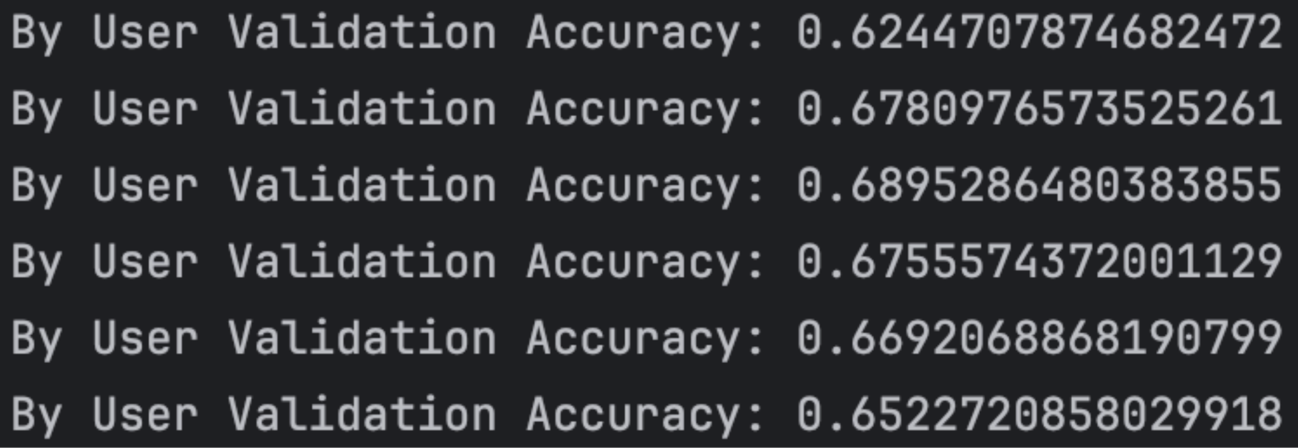
\includegraphics[width=5.8689in,height=2.0272in]{a0000-img001.png}}
\par

\bigskip


\lfbox[margin-bottom=0.0035in,margin-top=0mm,margin-right=0mm,margin-left=0mm,border-style=none,padding=0mm,vertical-align=top]{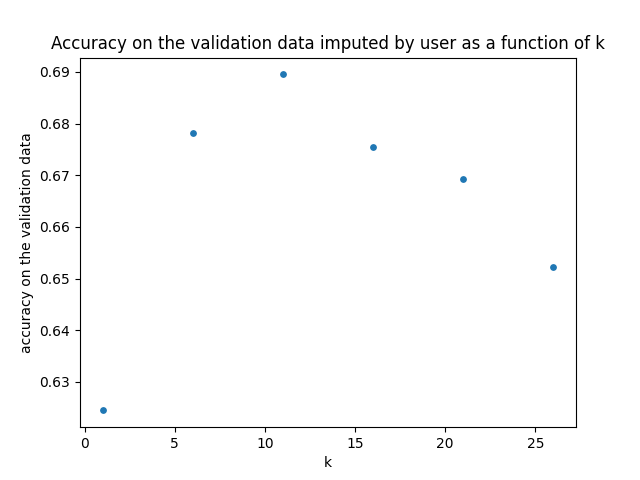
\includegraphics[width=5.922in,height=4.4417in]{a0000-img002.png}}



\bigskip

\textcolor{black}{\ We use k*=11 for }\textit{\textcolor{black}{knn\_imputed\_by\_user}}\textcolor{black}{ and the final
test accuracy is:}


\lfbox[margin=0mm,border-style=none,padding=0mm,vertical-align=top]{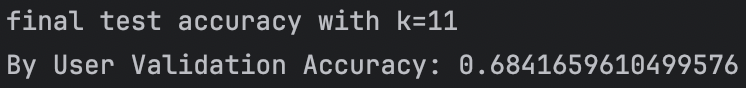
\includegraphics[width=5.1807in,height=0.611in]{a0000-img003.png}}


\begin{itemize}[series=listWWNumii,label=[F0B7?]]
\item \textbf{\textcolor{black}{Step 3:}}\textcolor{black}{ The fundamental premise of item-based collaborative
filtering is that if a diagnostic question A has the same number of correct and incorrect responses from other users as
question B, then the correctness of question A from a particular user is equal to that of question B.}
\end{itemize}
\textcolor{black}{The accuracy on validation data for k ${\in}$ \{1, 6, 11, 16, 21, 26\} is as the following:}


\lfbox[margin-bottom=0.0055in,margin-top=0mm,margin-right=0mm,margin-left=0mm,border-style=none,padding=0mm,vertical-align=top]{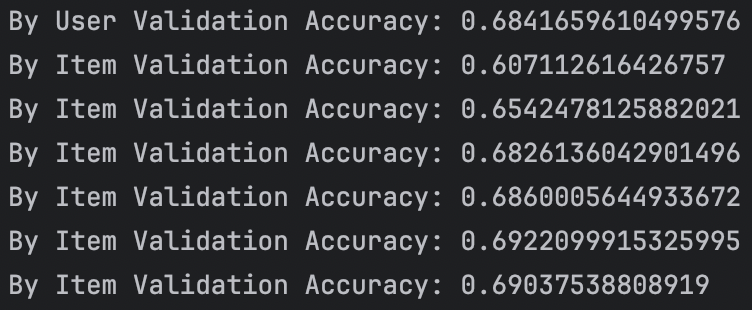
\includegraphics[width=5.3102in,height=2.1898in]{a0000-img004.png}}



\lfbox[margin=0mm,border-style=none,padding=0mm,vertical-align=top]{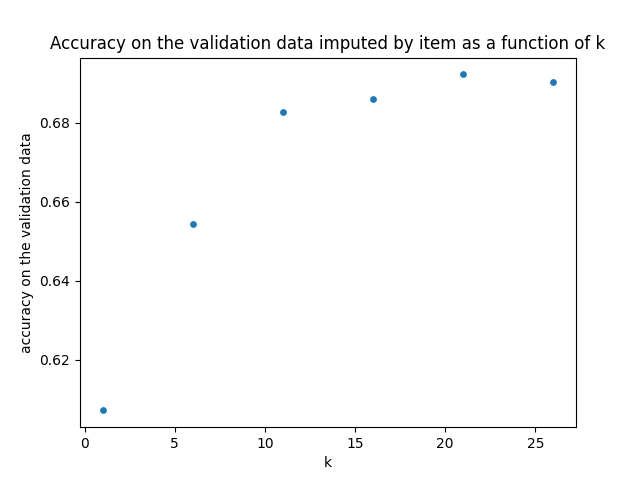
\includegraphics[width=5.3335in,height=4in]{a0000-img005.png}}


\textcolor{black}{We use k*=21 for }\textit{\textcolor{black}{knn\_imputed\_by\_item}}\textcolor{black}{ and the final
test accuracy is as following:}


\lfbox[margin=0mm,border-style=none,padding=0mm,vertical-align=top]{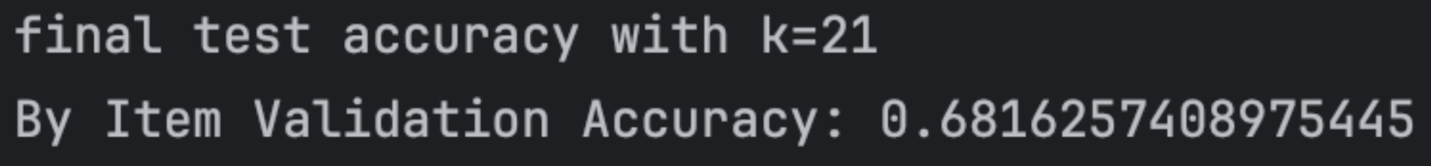
\includegraphics[width=6.5in,height=0.7555in]{a0000-img006.png}}


\begin{itemize}[series=listWWNumiii,label=[F0B7?]]
\item \textbf{\textcolor{black}{Step 4:}}\textcolor{black}{ The test performance between user- and item- collaborative
filtering is quite similar with user- based performs slightly better. Some reasons can be consider to lead to this
outcome:}
\end{itemize}
\textcolor{black}{+ Students might have consistent response patterns across questions}

\textcolor{black}{+ There could be clear groups of students with similar knowledge levels or learning styles}

\textcolor{black}{+ The number of students might be smaller than the number of questions, making user similarity more
reliable}

\textbf{4.2. Item Response Theory (IRT) }

\begin{itemize}[resume*=listWWNumii,start=1]
\item \textbf{Step 2:} Let n = total number of students and m = total number of questions. The log-likelihood is derived
as following under the Naive Bayes assumption: 
\end{itemize}
\begin{equation*}
\begin{matrix}p(C{\mid}\theta ,\beta )\wedge =p\left(c_{11},c_{12},\dots{},c_{\mathit{nm}}{\mid}\theta ,\beta
\right)\\\wedge =\prod _{i=1}^n\Box \prod _{j=1}^m\Box p\left(c_{\mathit{ij}}=1{\mid}\theta _i,\beta
_j\right)^{c_{\mathit{ij}}}{\cdot}\left(1-p\left(c_{\mathit{ij}}=1{\mid}\theta _i,\beta
_j\right)\right)^{\left(1-c_{\mathit{ij}}\right)}\\\wedge =\prod _{i=1}^n\Box \prod _{j=1}^m\Box \sigma \left(\theta
_i-\beta _j\right)^{c_{\mathit{ij}}}{\cdot}\left(1-\sigma \left(\theta _i-\beta
_j\right)\right)^{\left(1-c_{\mathit{ij}}\right)}\\\log \text{[2061?]}(p(C{\mid}\theta ,\beta ))\wedge =\log
\text{[2061?]}\left(\prod _{i=1}^n\Box \prod _{j=1}^m\Box \sigma \left(\theta _i-\beta
_j\right)^{c_{\mathit{ij}}}{\cdot}\left(1-\sigma \left(\theta _i-\beta
_j\right)\right)^{\left(1-c_{\mathit{ij}}\right)}\right)\\\wedge =\sum _{i=1}^n\Box \sum _{j=1}^m\Box
c_{\mathit{ij}}{\cdot}\log \text{[2061?]}\left(\sigma \left(\theta _i-\beta
_j\right)\right)+\left(1-c_{\mathit{ij}}\right){\cdot}\log \text{[2061?]}\left(1-\sigma \left(\theta _i-\beta
_j\right)\right)\end{matrix}
\end{equation*}
Now we calculate the partial derivative of the log-likelihood with respect to each $\theta $i and $\beta $j 

\begin{equation*}
\begin{matrix}\frac{{\partial}\log \text{[2061?]}(p(C{\mid}\theta ,\beta ))}{{\partial}\theta _i}=?\sum _{j=1}^m\Box
\frac{c_{\mathit{ij}}}{\sigma \left(\theta _i-\beta _j\right)}{\cdot}\frac{{\partial}\sigma \left(\theta _i-\beta
_j\right)}{{\partial}\left(\theta _i-\beta _j\right)}{\cdot}\frac{{\partial}\left(\theta _i-\beta
_j\right)}{{\partial}\theta _i}\\\frac{+1-c_{\mathit{ij}}}{1-\sigma \left(\theta _i-\beta
_j\right)}{\cdot}\frac{{\partial}\left(1-\sigma \left(\theta _i-\beta _j\right)\right)}{{\partial}\left(\theta _i-\beta
_j\right)}{\cdot}\frac{{\partial}\left(\theta _i-\beta _j\right)}{{\partial}\theta _i}\\?\end{matrix}
\end{equation*}
\begin{equation*}
\begin{matrix}\wedge \begin{matrix}=&\sum _{j=1}^m\Box \frac{c_{\mathit{ij}}}{\sigma \left(\theta _i-\beta
_j\right)}{\cdot}\sigma \left(\theta _i-\beta _j\right){\cdot}\left(1-\sigma \left(\theta _i-\beta
_j\right)\right){\cdot}1\\\frac{+1-c_{\mathit{ij}}}{1-\sigma \left(\theta _i-\beta _j\right)}{\cdot}-\sigma
\left(\theta _i-\beta _j\right){\cdot}\left(1-\sigma \left(\theta _i-\beta _j\right)\right){\cdot}1\end{matrix}\\\wedge
\text{ (We used }\left.\sigma ^{'}(x)=\sigma (x)(1-\sigma (x))\right)\\\wedge \begin{matrix}=\sum _{j=1}^m\Box
c_{\mathit{ij}}{\cdot}\left(1-\sigma \left(\theta _i-\beta _j\right)\right)-\left(1-c_{\mathit{ij}}\right){\cdot}\sigma
\left(\theta _i-\beta _j\right)\\=\sum _{j=1}^m\Box c_{\mathit{ij}}-c_{\mathit{ij}}{\cdot}\sigma \left(\theta _i-\beta
_j\right)-\sigma \left(\theta _i-\beta _j\right)+c_{\mathit{ij}}{\cdot}\sigma \left(\theta _i-\beta _j\right)\\=\sum
_{j=1}^m\Box c_{\mathit{ij}}-\sigma \left(\theta _i-\beta _j\right)\end{matrix}\end{matrix}
\end{equation*}

\bigskip

\begin{equation*}
\begin{matrix}\wedge \frac{{\partial}\log \text{[2061?]}(p(C{\mid}\theta ,\beta ))}{{\partial}\beta _j}=\sum
_{i=1}^n\Box \frac{c_{\mathit{ij}}}{\sigma \left(\theta _i-\beta _j\right)}{\cdot}\frac{{\partial}\sigma \left(\theta
_i-\beta _j\right)}{{\partial}\left(\theta _i-\beta _j\right)}{\cdot}\frac{{\partial}\left(\theta _i-\beta
_j\right)}{{\partial}\beta _j}\\\wedge +\frac{1-c_{\mathit{ij}}}{1-\sigma \left(\theta _i-\beta
_j\right)}{\cdot}\frac{{\partial}\left(1-\sigma \left(\theta _i-\beta _j\right)\right)}{{\partial}\left(\theta _i-\beta
_j\right)}{\cdot}\frac{{\partial}\left(\theta _i-\beta _j\right)}{{\partial}\beta _j}\\\wedge =\sum _{i=1}^n\Box
\frac{c_{\mathit{ij}}}{\sigma \left(\theta _i-\beta _j\right)}{\cdot}\sigma \left(\theta _i-\beta
_j\right){\cdot}\left(1-\sigma \left(\theta _i-\beta _j\right)\right){\cdot}-1\\\wedge
+\frac{1-c_{\mathit{ij}}}{1-\sigma \left(\theta _i-\beta _j\right)}{\cdot}-\sigma \left(\theta _i-\beta
_j\right){\cdot}\left(1-\sigma \left(\theta _i-\beta _j\right)\right){\cdot}-1\\\wedge \left(\text{ We used }\sigma
^{'}(x)=\sigma (x)(1-\sigma (x))\right)\\\wedge =\sum _{i=1}^n\Box -c_{\mathit{ij}}{\cdot}\left(1-\sigma \left(\theta
_i-\beta _j\right)\right)+\left(1-c_{\mathit{ij}}\right){\cdot}\sigma \left(\theta _i-\beta _j\right)\\\wedge =\sum
_{i=1}^n\Box -c_{\mathit{ij}}+c_{\mathit{ij}}{\cdot}\sigma \left(\theta _i-\beta _j\right)+\sigma \left(\theta _i-\beta
_j\right)-c_{\mathit{ij}}{\cdot}\sigma \left(\theta _i-\beta _j\right)\\\wedge =\sum _{i=1}^n\Box
-c_{\mathit{ij}}+\sigma \left(\theta _i-\beta _j\right)\end{matrix}
\end{equation*}
\begin{itemize}[resume*=listWWNumii]
\item \textbf{Step 3:} To achieve a stable training curve we adjust learning rate and the number of iterations as the
following:
\end{itemize}

\lfbox[margin-right=0.002in,margin-top=0mm,margin-bottom=0mm,margin-left=0mm,border-style=none,padding=0mm,vertical-align=top]{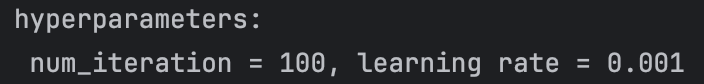
\includegraphics[width=4.5681in,height=0.5453in]{a0000-img007.png}}


\ \ \ \ Negative log-likelihood in each interaction for the training set: 


\lfbox[margin=0mm,border-style=none,padding=0mm,vertical-align=top]{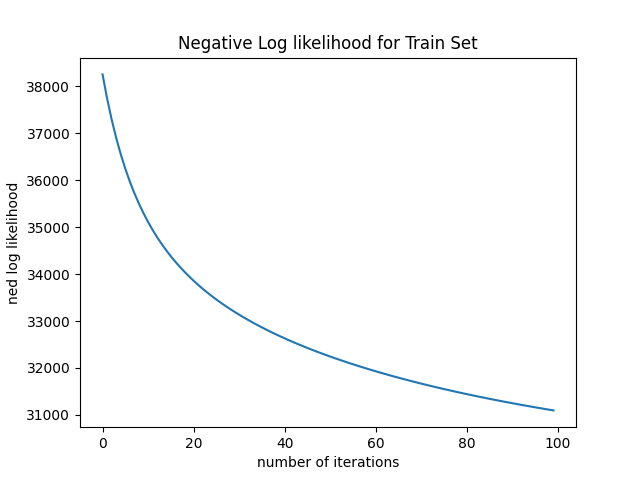
\includegraphics[width=4.7807in,height=3.5854in]{a0000-img008.png}}


\ \ \ \ Negative log-likelihood in each interaction for the validation set: 


\lfbox[margin=0mm,border-style=none,padding=0mm,vertical-align=top]{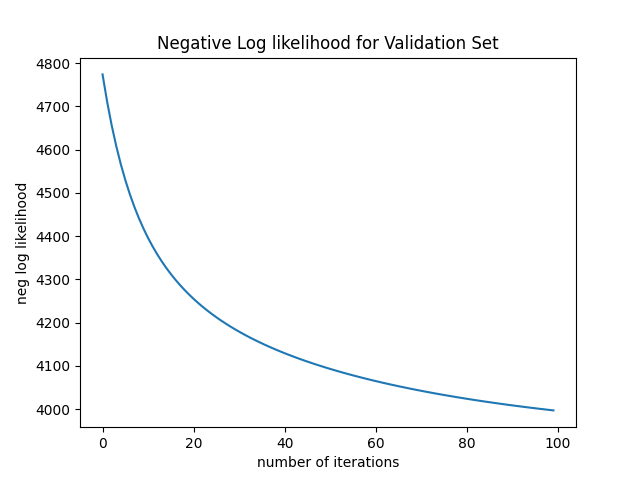
\includegraphics[width=4.7807in,height=3.5854in]{a0000-img009.png}}


\begin{itemize}[resume*=listWWNumii]
\item \textbf{Step 4:} Plot for the probability of getting correct response vs theta for 3 questions: 
\end{itemize}

\lfbox[margin=0mm,border-style=none,padding=0mm,vertical-align=top]{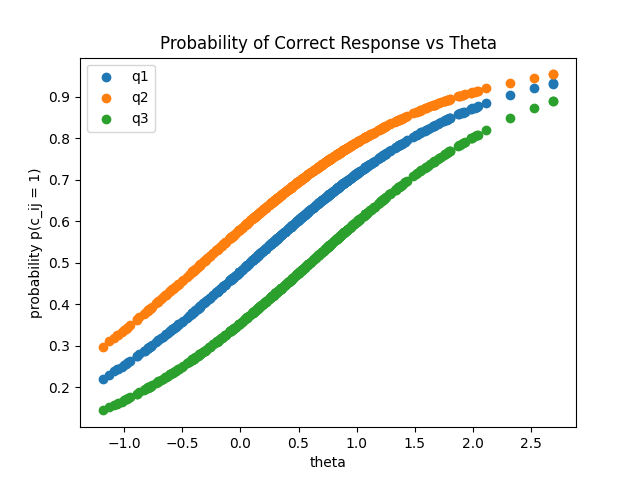
\includegraphics[width=6.389in,height=4.7917in]{a0000-img010.png}}


\begin{itemize}[resume*=listWWNumii]
\item \textbf{Step 5:} From this graph, we observe that when theta is small, the probability of correct responses is
low, and as theta increases, the probability of correct responses also increases. This makes sense because theta
represents a student's ability. Students with lower ability are less likely to answer correctly, while those with
higher ability are more likely to do so. The three curves in the graph roughly follow an S-shape, as we used the
sigmoid function $\sigma $($\theta $ $-$ $\beta $) to calculate the probability. As $\theta $ increases, the input to
the sigmoid, $\theta $ $-$ $\beta $, also increases. Since the sigmoid is a monotonically increasing function with an
S-shape, the probability follows a similar pattern. The vertical displacement of the three curves could represent
different levels of question difficulty. For easier questions, students of all abilities are more likely to get them
right, whereas for harder questions, students of all abilities are more likely to get them wrong.
\end{itemize}

\bigskip


\bigskip


\bigskip


\bigskip

\textbf{4.3: Ensemble Learning}

In this section, we implemented a bagging ensemble method using the Item Response Theory (IRT) algorithm to enhance the
accuracy and stability of our base models. The process consists of the following steps:

\begin{itemize}[resume*=listWWNumii]
\item \textbf{Step 1:} Data Resampling\newline
We created three new training sets by resampling from the original dataset. Each of these sets was generated by randomly
selecting samples with replacement, ensuring that they contained the same number of samples as the original dataset.
\item \textbf{Step 2:} Model Predictions\newline
For each resampled training set, we computed the predictions yiy\_iyi\hspace{0pt} using the respective training set i.
\item \textbf{Step 3:} Averaging Predictions\newline
We then calculated the average prediction as follows:\newline
 $y=\frac 1 3\sum _{i=1}^3y_i$
\end{itemize}
\newline
Given that this task involves binary classification (determining whether student i answered question j correctly), we
applied a threshold of 0.5 to derive the final prediction:\newline
 $y_{\mathit{bagged}}=I\left(\frac 1 3\sum _{i=1}^3y_i>0.5\right)$


\bigskip

\begin{itemize}[resume*=listWWNumii]
\item \textbf{Step 4:} Performance Evaluation\newline
Finally, we compared the ensemble predictions with the validation data to calculate the accuracy of the ensemble model.
\end{itemize}

\bigskip

\textbf{Final Results}

The hyperparameters used included 280 iterations and a learning rate of 0.0005.


\lfbox[margin=0mm,border-style=none,padding=0mm,vertical-align=top]{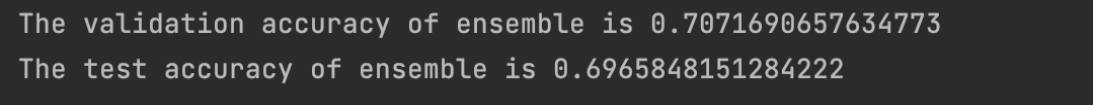
\includegraphics[width=5.7165in,height=0.6307in]{a0000-img011.png}}



\bigskip

\textbf{Performance Assessment\newline
}The validation accuracy for the ensemble was slightly lower than that of the individual base models, while the test
accuracy remained unchanged. It is worth noting that the gap between validation and test accuracy for the ensemble was
smaller compared to the original model, indicating that the ensemble approach provided greater prediction stability.

While bagging typically helps average out various sources of noise in the data, thus reducing variance, it does not
alter the bias or Bayes error. Theoretically, using an ensemble model should lead to improved accuracy; however, in our
case, the use of only three base models may not have been sufficient to achieve a significant boost in performance.
Consequently, our test accuracy did not see any improvement.


\bigskip

\textbf{4.4. Matrix Factorization}

\begin{itemize}[resume*=listWWNumii]
\item \textbf{Step 1:} Singular value decomposition (SVD)
\end{itemize}

\bigskip

We implemented SVD to factorize the response matrix into two smaller matrices representing latent factors for students
and questions. For the latent dimension k, we tried five distinct values:  $k=\left\{7,14,21,56,105\right\}$. 

The validation accuracies for each k value are as follows: 


\lfbox[margin-right=0.0016in,margin-bottom=0.0028in,margin-top=0mm,margin-left=0mm,border-style=none,padding=0mm,vertical-align=top]{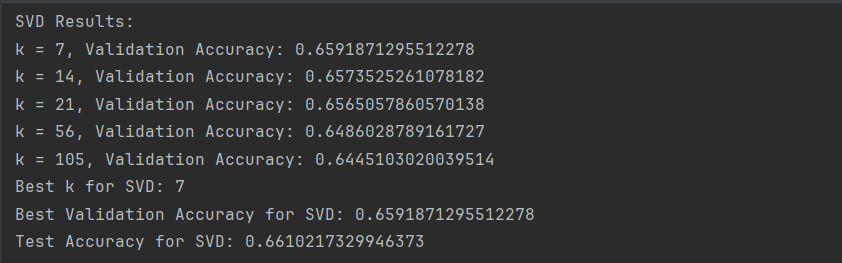
\includegraphics[width=6.728in,height=2.1016in]{a0000-img012.png}}


The best k for SVD was found to be 7, and both the test and validation accuracy were approximately 0.66.


\bigskip

We also plot the results in the following figure:\newline

\lfbox[margin-right=0.0016in,margin-bottom=0.0047in,margin-top=0mm,margin-left=0mm,border-style=none,padding=0mm,vertical-align=top]{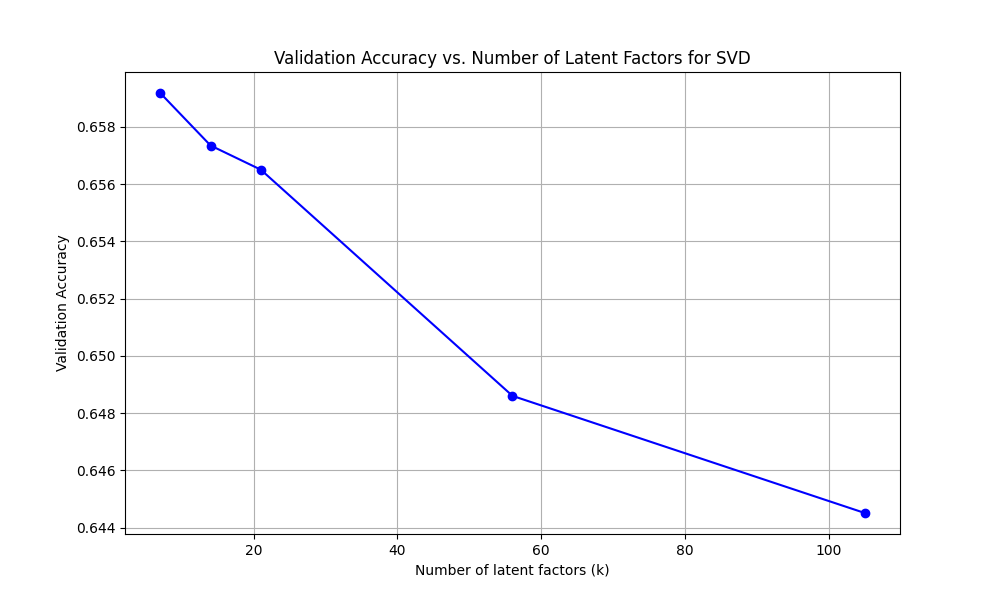
\includegraphics[width=6.728in,height=4.0366in]{a0000-img013.png}}


{\centering
Figure 1. The validation accuracy versus the number of latent factors for the SVD method.
\par}

This graph shows how the validation accuracy changes with the number of latent factors for the SVD method. The accuracy
is highest at the lowest number of factors (around  $k=7$) and steadily decreases as the number of factors increases.
This suggests that for SVD, simpler models (with fewer latent factors) perform better on the validation set, possibly
due to better generalization.


\bigskip

\begin{itemize}[resume*=listWWNumii]
\item Step 2: Alternating least square (ALS)
\end{itemize}

\bigskip

In this step, the ALS is implemented using stochastic gradient descent (SGD) by first initializing and iteratively
updating the user (U) and question (Z) matrices randomly through the function \textit{update\_u\_z().} Then we use this
function in the \textit{als()} function to run the entire process. We also use the same set of latent dimensions k in
this step \  $k=\left\{7,14,21,56,105\right\}$. We also use different values for the learning rate lr 
$\mathit{lr}=\left\{0.01,0.1,0.25,0.5\right\}$ \ to look for promising convergence time and the vali dation accuracy
decreased without any fluctuation (unlike some larger learning rates). The \textit{lr }value we choose is 0.1. 


\bigskip

The validation accuracies for each k value are as follows: 


\lfbox[margin-right=0.0016in,margin-bottom=0.0043in,margin-top=0mm,margin-left=0mm,border-style=none,padding=0mm,vertical-align=top]{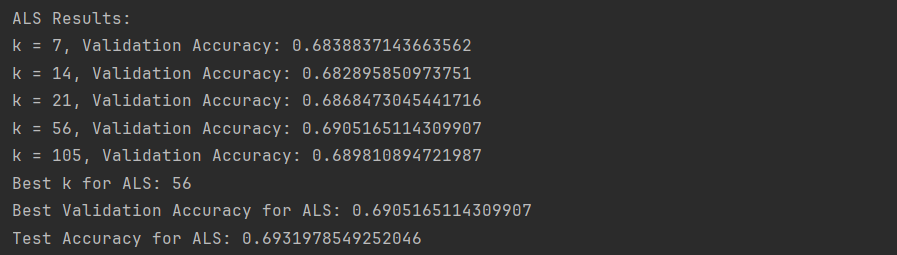
\includegraphics[width=6.728in,height=1.9126in]{a0000-img014.png}}


{\centering
Figure 2. The ALS validation accuracies for each k values
\par}


\bigskip

The best k for ALS was found to be 56, with the validation accuracy to be nearly 0.69 and the test accuracy to be
approximately 0.693.


\bigskip

The following figure shows the relationship between the validation accuracy and the number of latent factors (k) for the
ALS method.


\lfbox[margin-right=0.0016in,margin-bottom=0.0047in,margin-top=0mm,margin-left=0mm,border-style=none,padding=0mm,vertical-align=top]{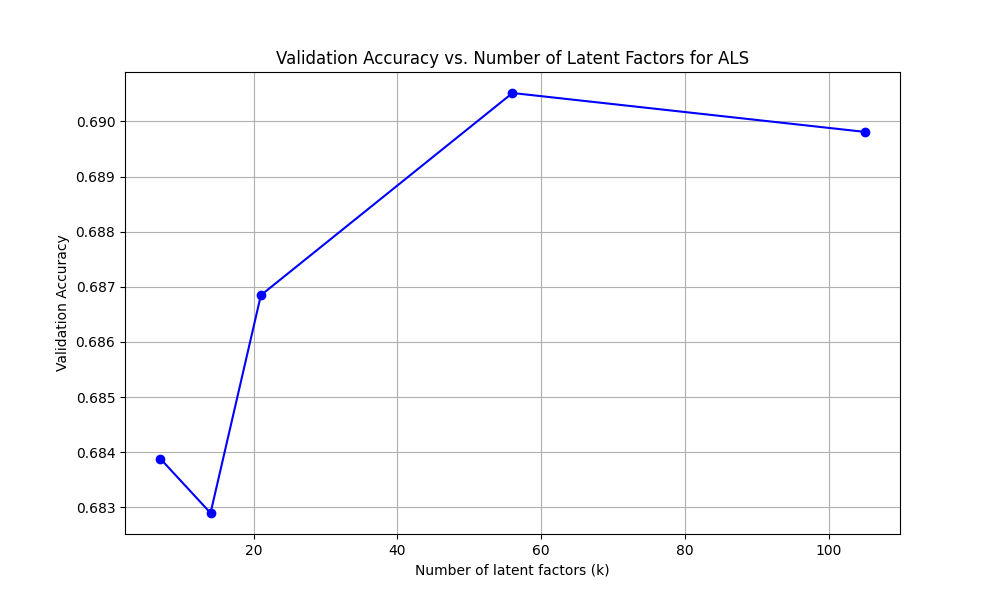
\includegraphics[width=6.728in,height=4.0366in]{a0000-img015.png}}


{\centering
Figure 3. The validation accuracies versus the number of latent factors for the ALS.
\par}


\bigskip

The peak accuracy appears to occur around  $k=56$, with a validation accuracy of approximately 0.6905. After this peak,
there's a slight decrease in accuracy as k increases to 100, but the decline is minimal.


\bigskip

We also have the following figure to present the training losses and validation losses in each iteration of the best k: 


\lfbox[margin-right=0.0016in,margin-bottom=0.0055in,margin-top=0mm,margin-left=0mm,border-style=none,padding=0mm,vertical-align=top]{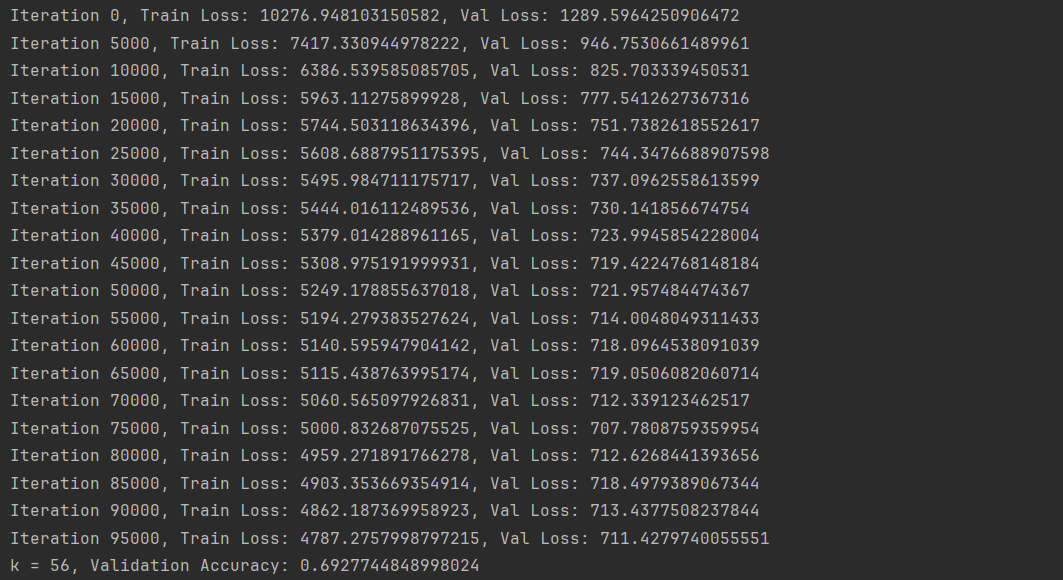
\includegraphics[width=6.7071in,height=3.661in]{a0000-img016.png}}


{\centering
Figure 4. The training losses and validation losses in each iteration of  $k=56$.
\par}


\lfbox[margin-right=0.0016in,margin-bottom=0.0047in,margin-top=0mm,margin-left=0mm,border-style=none,padding=0mm,vertical-align=top]{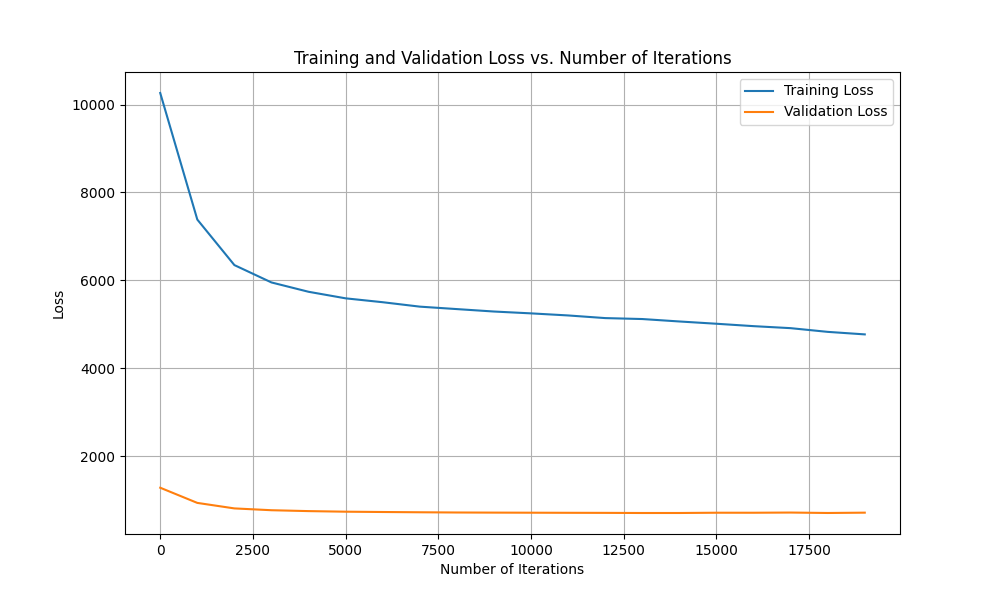
\includegraphics[width=6.728in,height=4.0366in]{a0000-img017.png}}


{\centering
Figure 5. The training and validation loss versus the number of iterations for the ALS method.
\par}


\bigskip

This figure illustrates how the training and validation losses change with the number of iterations in the machine
learning model. The training loss (blue line) starts very high, and consistently decreases as the number of iterations
increases, indicating that the model is learning from the training data. The rate of decrease is rapid initially and
then becomes more gradual.

The validation loss (orange line) starts much lower, around 1,500, and also decreases, but at a much slower rate
compared to the training loss. It seems to remain unchanged after about 5,000 iterations, with only minimal changes
afterwards. This suggests that the model's performance on unseen data stabilizes relatively early in the training
process.

The continuing decrease in training loss, coupled with the relatively stable validation loss, indicates that the model
is improving its fit to the training data without significant overfitting to the validation set.


\bigskip

\begin{itemize}[resume*=listWWNumii]
\item \textbf{Step 3:}
\end{itemize}

\bigskip

1. Comparison of SVD and ALS

We compared the results of SVD and ALS by plotting the validation accuracies for both methods against the number of
latent factors (k). This comparison is visualized in the following figure:


\lfbox[margin-right=0.0016in,margin-bottom=0.0047in,margin-top=0mm,margin-left=0mm,border-style=none,padding=0mm,vertical-align=top]{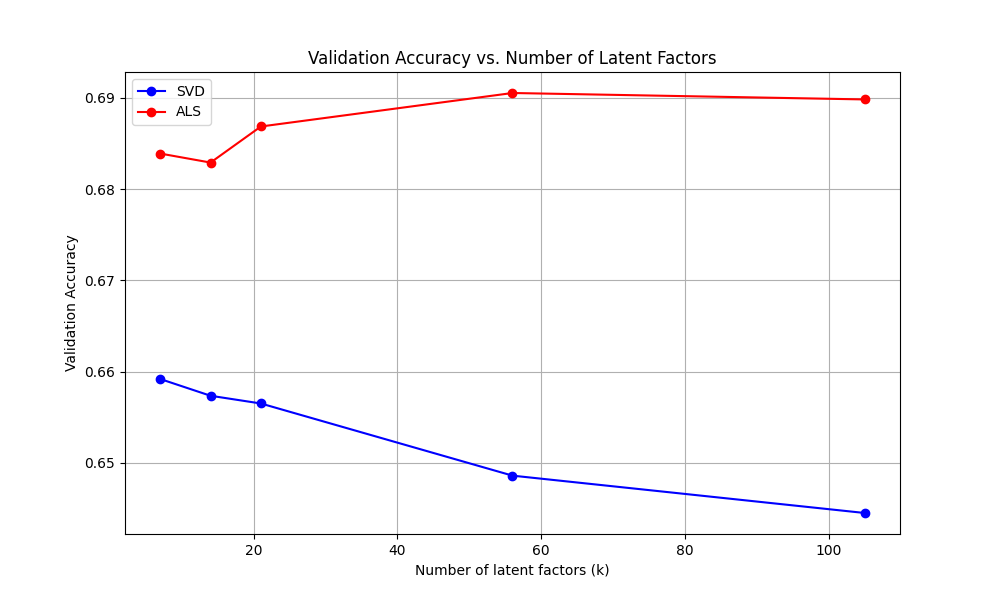
\includegraphics[width=6.728in,height=4.0366in]{a0000-img018.png}}


{\centering
Figure 6. The validation accuracy versus the number of latent factors for both SVD (Singular Value Decomposition) and
ALS methods.
\par}


\bigskip

This figure compares the validation accuracy of two methods, SVD (Singular Value Decomposition) and ALS (Alternating
Least Squares), across different numbers of latent factors. 

The ALS method consistently outperforms SVD across all numbers of latent factors. The ALS line shows a general upward
trend as the number of latent factors increases, with a slight dip around 20 factors. It reaches its peak around 60
factors and then plateaus.

The SVD line shows a downward trend as the number of latent factors increases, starting at its highest point with 10
factors and declining steadily.

For both methods, the validation accuracy stays within a relatively narrow range (approximately 0.645 to 0.69),
suggesting that changing the number of latent factors has a limited impact on overall performance.


\bigskip


\bigskip

2. Limitation of Matrix Factorization

\begin{itemize}[series=listWWNumvii,label=[F0B7?]]
\item Handling of Missing Data: In the SVD implementation, we filled in missing values using the average of the current
item. This approach may introduce bias, especially if the missing data is not randomly distributed.
\item Cold Start Problem: Matrix factorization methods may struggle with new users or items that have no or very few
ratings, as there isn't enough information to accurately place them in the latent space.
\item Interpretability: The latent factors discovered by these methods are not always easily interpretable, making it
challenging to explain why certain predictions are made.
\item Scalability: As the number of users and items grows, the computational cost of these methods can increase
significantly, especially for larger values of k.
\item Assumption of Linearity: These methods assume that the interaction between user and item factors is linear, which
may not always hold true in real-world scenarios.
\item Temporal Dynamics: Standard matrix factorization doesn't account for changes in user preferences or item
characteristics over time, which could be relevant in an educational context where student knowledge evolves.
\end{itemize}

\bigskip

\clearpage
\textbf{\textcolor{black}{Part B: Algorithm Modification}}

\textbf{Based on the results from Part A, In Part B}, we chose the Item Response Theory (IRT) algorithm to extend and
improve prediction accuracy.


\bigskip

\textbf{Identify the modification you are making and why it is expected to improve performance}


\bigskip

\textbf{• Extension 1: Add parameter $\alpha [2C7C?]$ to describe the discriminative power of the question}

In the original model, there is a simplified assumption that the probability of answering correctly depends only on two
parameters:

\begin{itemize}[series=listWWNumx,label=[F0B7?]]
\item \textbf{$\theta [1D62?]$}: the ability of student i
\item \textbf{$\beta [2C7C?]$}: the difficulty of question j.
\end{itemize}
However, assuming that all questions are equally discriminative may not hold true in practice. Therefore, we decided to
introduce the parameter \textbf{$\alpha [2C7C?]$} to describe the discriminative power of each question.

Figure 5 in the Figures/Charts section illustrates how different values of \textbf{$\alpha $} affect the probability of
answering correctly. When \textbf{x} is negative, the blue line is lower than the red line; when \textbf{x} is
positive, the blue line is higher than the red line. This indicates that students with lower ability are less likely to
answer highly discriminative questions correctly, and vice versa.

We add \textbf{$\alpha $} to the model, compute the derivative of the log-likelihood function with respect to
\textbf{$\alpha [2C7C?]$}, and apply gradient descent on \textbf{$\alpha $} similarly to \textbf{$\theta $} and
\textbf{$\beta $} to optimize the log-likelihood function. Additionally, we constrain \textbf{$\alpha $} to the range
(0,2) since this is a more realistic range as suggested by Columbia Public Health. For further details, refer to the
IRT theory.

\textbf{• Extension 2: Add a hyperparameter c describing the probability of guessing the correct answer}

We assume that all questions are multiple-choice with 4 options (as in the example diagnostic question provided in the
materials). Given that students may guess when they do not know the answer, we decided to add a hyperparameter
\textbf{c} to the model. After tuning, the optimal value of \textbf{c} is 0.25.

After this extension, our probability function becomes:

\begin{equation*}
P(\mathit{c\text{[1D62?]}\text{[2C7C?]}}\vee \mathit{\theta \text{[1D62?]}},\mathit{\beta \text{[2C7C?]}})=c+[1-c]\times
\mathit{sigmoid}(\mathit{\alpha \text{[2C7C?]}}(\mathit{\theta \text{[1D62?]}}-\mathit{\beta \text{[2C7C?]}}))
\end{equation*}
This extended model introduces two additional factors: the discriminative power of questions and the chance of students
guessing, adding complexity and better capturing the characteristics of the dataset. Therefore, we expect our extended
model to improve optimization and achieve higher test accuracy.


\bigskip


\bigskip

\textbf{Evaluate the accuracy of the algorithm}

Our hypothesis is that adding parameters \textbf{$\alpha $} and \textbf{c} will improve performance because it increases
the model's complexity, allowing it to capture more characteristics of the dataset. To test this hypothesis, we will
implement the modified model as described earlier and run it on the dataset to evaluate its performance. (The code for
this section can be found in {\textbackslash}part a{\textbackslash}part2 irt.py).

We chose three models to compare the performance of the modified algorithm: the original IRT model, the modified IRT
model with \textbf{c = 0} (representing no random guessing), and the modified IRT model with \textbf{c = 0.25}
(representing a 25\% chance of answering a question correctly through random guessing).

For a set of 9 different hyperparameter combinations, which consist of loop iterations  $\{100,150,200\}$ \ and learning
rates  $\{0.0025,0.001,0.0005\}$, we find the best validation accuracy each model can achieve. The validation
accuracies are summarized in the table below: 


\bigskip

\begin{flushleft}
\tablefirsthead{\hline
\multicolumn{10}{|m{6.976159in}|}{\centering Iterations}\\}
\tablehead{\hline
\multicolumn{10}{|m{6.976159in}|}{\centering Iterations}\\}
\tabletail{}
\tablelasttail{}
\begin{supertabular}{|m{0.59555984in}|m{0.5906598in}|m{0.6504598in}|m{0.6497598in}|m{0.5906598in}|m{0.6504598in}|m{0.6497598in}|m{0.5906598in}|m{0.6504598in}|m{0.64905983in}|}
\hline
~
 &
\multicolumn{3}{m{2.0483599in}|}{\centering 100} &
\multicolumn{3}{m{2.0483599in}|}{\centering 150} &
\multicolumn{3}{m{2.0476599in}|}{\centering 200}\\\hline
\centering learning rate &
\centering original irt &
{\centering modified irt,\par}

\centering c= 0 &
{\centering modified irt,\par}

\centering c= 0.25 &
\centering original irt &
{\centering modified irt,\par}

\centering c= 0 &
{\centering modified irt,\par}

\centering c= 0.25 &
\centering original irt &
{\centering modified irt,\par}

\centering c= 0 &
{\centering modified irt,\par}

\centering\arraybslash c= 0.25\\\hline
\centering 0.0025 &
\centering 0.70759 &
\centering 0.70745 &
\centering 0.70900 &
\centering 0.70590 &
\centering 0.70787 &
\centering 0.70759 &
\centering 0.70562 &
\centering 0.70687 &
\centering\arraybslash 0.70703\\\hline
\centering 0.001 &
\centering 0.70745 &
\centering 0.70886 &
\centering 0.69433 &
\centering 0.70802 &
\centering 0.70844 &
\centering 0.70447 &
\centering 0.70675 &
\centering 0.70773 &
\centering\arraybslash 0.70900\\\hline
\centering 0.0005 &
\centering 0.69785 &
\centering 0.69574 &
\centering 0.67556 &
\centering 0.70745 &
\centering 0.70590 &
\centering 0.68882 &
\centering 0.70745 &
\centering 0.70872 &
\centering\arraybslash 0.69461\\\hline
\end{supertabular}
\end{flushleft}

\bigskip

As observed from the table, the maximum validation accuracy achieved by the modified model with \textbf{c = 0.25}
(0.70900) is higher than that achieved by the modified model with \textbf{c = 0} (0.70886). Additionally, both modified
models perform better than the original model, which achieved a maximum validation accuracy of 0.70802


\bigskip

.
\lfbox[margin-bottom=0.0098in,margin-top=0mm,margin-right=0mm,margin-left=0mm,border-style=none,padding=0mm,vertical-align=top]{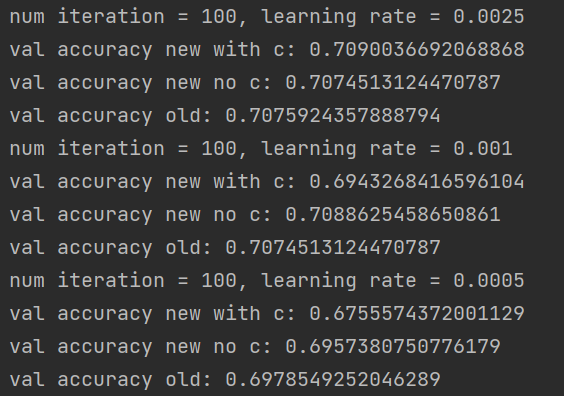
\includegraphics[width=2.0665in,height=1.4693in]{a0000-img019.png}}
 
\lfbox[margin-right=0.0063in,margin-bottom=0.0075in,margin-top=0mm,margin-left=0mm,border-style=none,padding=0mm,vertical-align=top]{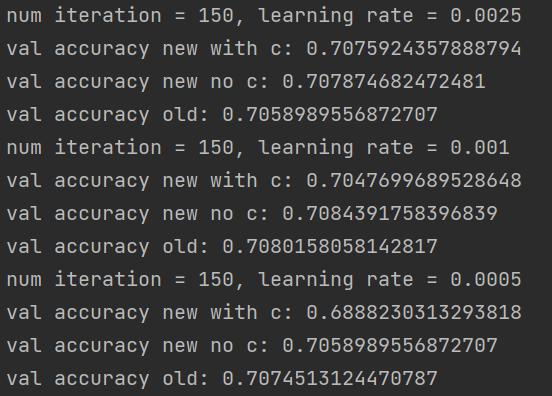
\includegraphics[width=2.0362in,height=1.4717in]{a0000-img020.png}}
\ \ 
\lfbox[margin-bottom=0.0063in,margin-top=0mm,margin-right=0mm,margin-left=0mm,border-style=none,padding=0mm,vertical-align=top]{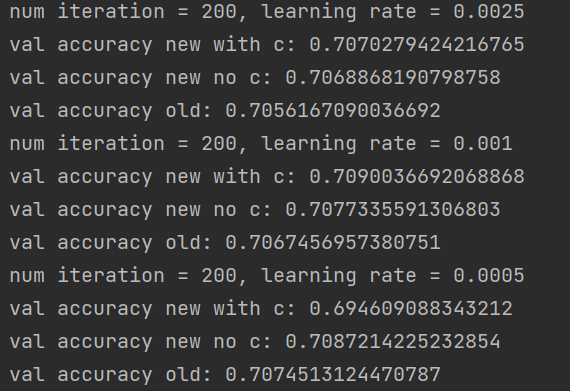
\includegraphics[width=2.1319in,height=1.4736in]{a0000-img021.png}}


This demonstrates that adding parameters \textbf{$\alpha $} and \textbf{c} contributes to performance improvement in
some aspects. 


\lfbox[margin=0mm,border-style=none,padding=0mm,vertical-align=top]{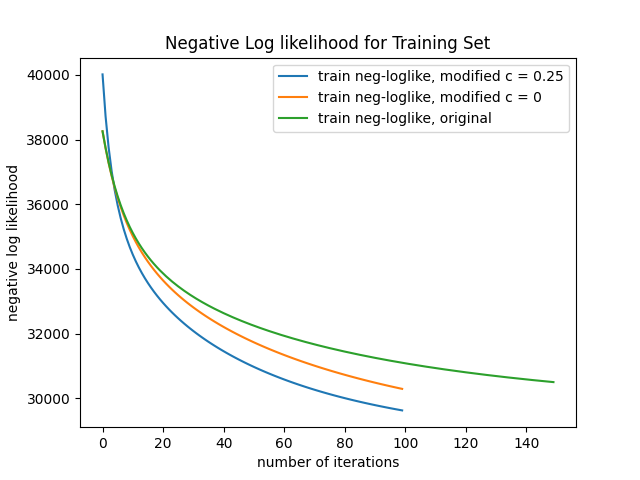
\includegraphics[width=3.0626in,height=2.3126in]{a0000-img022.png}}

\lfbox[margin-right=0.0102in,margin-top=0mm,margin-bottom=0mm,margin-left=0mm,border-style=none,padding=0mm,vertical-align=top]{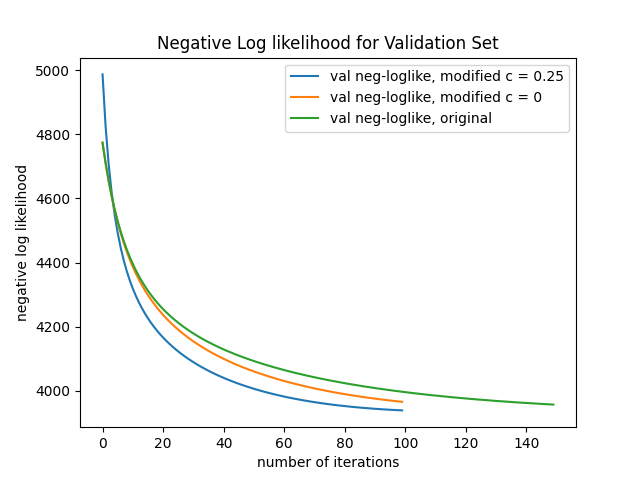
\includegraphics[width=3.0937in,height=2.3126in]{a0000-img023.png}}


By examining the changes in negative log-likelihood across iterations for both the training and validation sets, we can
observe the correspondence between the negative log-likelihood curves and validation accuracies for different models
shown in the table. For instance, the negative log-likelihood of the modified model with \textbf{c = 0.25} is lower
than the other two curves for most iterations, indicating that the prediction likelihood of this modified model is
higher. This is consistent with the model having the highest validation accuracy.

The test accuracies for all three models also show improved performance for the modified model with \textbf{c = 0.25}. 


\bigskip


\lfbox[margin-bottom=0.0102in,margin-top=0mm,margin-right=0mm,margin-left=0mm,border-style=none,padding=0mm,vertical-align=top]{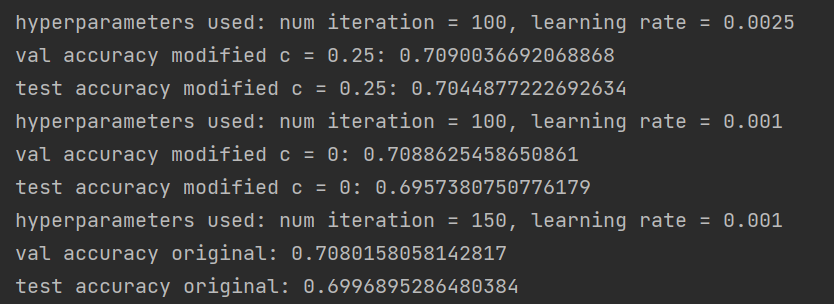
\includegraphics[width=6.2709in,height=2.2811in]{a0000-img024.png}}



\bigskip

However, the increase in validation accuracy is not substantial. For the modified model with \textbf{c = 0.25}, the
slight improvement in accuracy suggests that our assumption of all questions being multiple-choice with four options
may not have been ideal. Using a uniform \textbf{c} value could have limited further improvements, as different
questions may have varying numbers of answer choices.


\bigskip


\bigskip


\bigskip

\textbf{Visualization}


\bigskip


\lfbox[margin=0mm,border-style=none,padding=0mm,vertical-align=top]{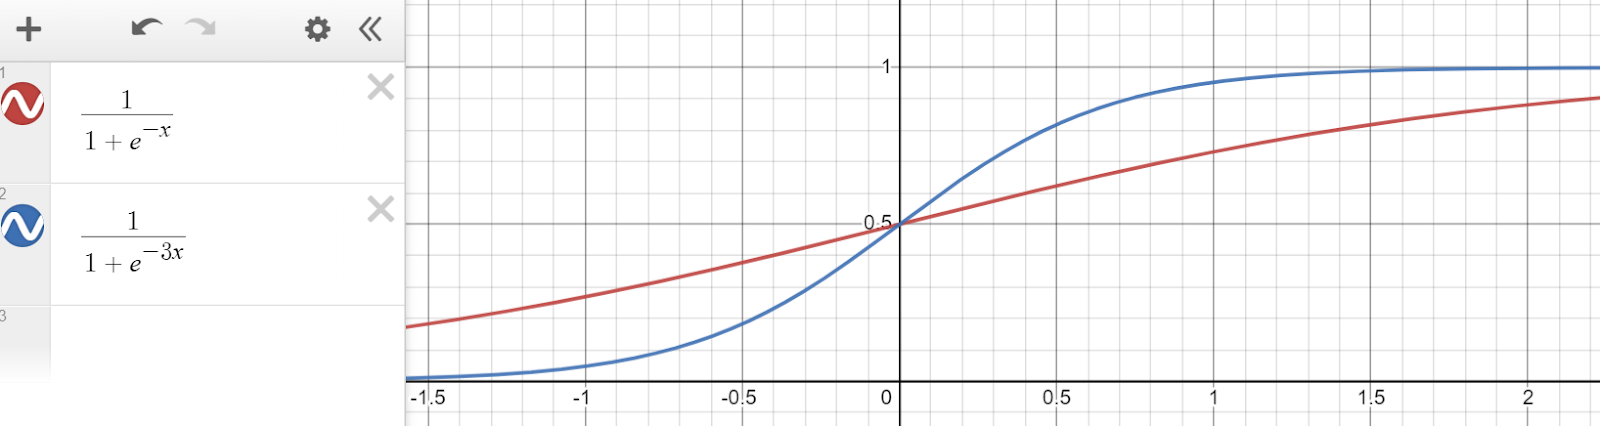
\includegraphics[width=6.2709in,height=1.6665in]{a0000-img025.png}}


{\centering
\textit{Figure 5: Probability of correct response for different $\alpha $ value}
\par}


\bigskip


\bigskip


\bigskip

\clearpage
\textbf{Limitations and potential improvements}

Although our extended IRT model has achieved good validation and test accuracies, there are several limitations that
affect its performance in certain situations. Below, we summarize these limitations and propose potential extensions to
address them.


\bigskip

\begin{itemize}[series=listWWNumxi,label=[F0B7?]]
\item \textbf{Assumption of Uniform Multiple-Choice Structure}: In this project, we lacked specific information on how
many answer options were present for each multiple-choice question. We assumed that all questions had four options with
only one correct answer, which might not always hold true. This assumption led us to set a uniform hyperparameter
\textbf{c} (with a value of 0.25 for four options), which could be inappropriate if different questions have varying
numbers of answer choices. A poor choice of \textbf{c} may cause underfitting when the data includes questions with
different option counts. A possible improvement is to replace the scalar \textbf{c} with a vector 
$c=(c\text{[2081?]},...,\mathit{c\text{[2099?]}}\text{[208D?]}\mathit{questions}\text{[208E?]})$, where each
\textbf{c[2C7C?]} represents the probability of guessing the correct answer for question \textbf{j}, thus accounting
for variable numbers of options across questions.
\end{itemize}

\bigskip

\begin{itemize}[resume*=listWWNumxi]
\item \textbf{Limited Generalization to Non-Multiple-Choice Questions}: All four models (KNN, IRT, NN, and ensemble)
were trained on datasets containing only multiple-choice questions. As a result, these models are expected to perform
poorly on datasets with other question types, such as short-answer or fill-in-the-blank questions. Instead of assuming
a binary outcome (correct/incorrect) for all questions, one possible extension is to adapt the model for polytomous
outcomes, where responses can receive partial credit and be rated on a scale (e.g., 1-5). This would allow the model to
handle a wider range of question types more effectively.
\end{itemize}

\bigskip

\begin{itemize}[resume*=listWWNumxi]
\item \textbf{Single Ability Value Limitation}: In our current IRT model, each student \textbf{i} is assigned a single
ability score \textbf{$\theta [1D62?]$}. Predictions on whether a student can answer question \textbf{j} correctly
depend solely on their overall ability  $\mathit{\theta \text{[1D62?]}}$, the difficulty  $\mathit{\beta
\text{[2C7C?]}}$, and the discriminative power \textbf{$\alpha [2C7C?]$} of the question. This approach fails to
account for a student's varying ability across different subjects or topics. For example, a student may excel in most
subjects but struggle with specific areas, such as multivariable calculus. Despite their overall high ability score
\textbf{$\theta [1D62?]$}, the model may overestimate their likelihood of answering a calculus question correctly. To
address this issue, we could introduce an ability matrix \textbf{$\theta $}, where  $\mathit{\theta
\text{[1D62?]}},\text{[2099?]}$ \ represents the student's ability in subject \textbf{n}. This matrix could be
initialized using the provided metadata and refined based on the student's performance on subject-specific questions.
By normalizing the matrix and incorporating it into the probability calculation, we could improve the
model$\text{\textgreek{’}}$s ability to predict performance across diverse subjects. The updated probability for a
student answering a question correctly would then be based on their specific abilities in the relevant subject areas,
increasing the overall accuracy of the model.
\end{itemize}

\bigskip


\bigskip
\end{document}
